\twocolumn[\begin{@twocolumnfalse}
	\chapter{Making a Printer cable\hfill\difficulty{3}}
	 The NABU Personal Computer \texttt{PRINTER} port allows printers with Centronics (parallel) interfaces to be connected. Since the NABU port features a non-standard parallel port connector, a custom cable is required. This section describes how to wire a cable with a DB-15 connector to a 36-way Centronics printer connector.
	\vskip1em
\end{@twocolumnfalse}]

\section{NABU Printer cable wiring}
The \texttt{PRINTER} port on the back of the NABU Personal Computer implements a parallel interface. The cable must be connected as specified in Table~\ref{tbl:kbdadaptor}. For best performance, the cable should be shielded.

\begin{center}
	\sffamily
	\begin{tblr}{
			colspec={|cccc|},
			cell{1}{1} = {c=2}{c},
			cell{1}{3} = {c=2}{c},
			row{1} = {font=\bfseries},
			row{1,2} = {bg=gray4,fg=white},
			row{4,6,8,10,12} = {bg=gray9},
			vline{3} = {3-13}{text=\clap{$\leftrightarrow$}},
			hline{1,3,14} = {solid}
		}
		NABU (DB-15) & & Printer (Centronics) &\\
		Signal & Pin & Pin & Signal \\
		$\mathsf{\overline{Strobe}}$ & 1 & 1 & $\mathsf{\overline{Strobe}}$ \\
		Data 0 & 2 & 2 & Data 0 \\
		Data 1 & 3 & 3 & Data 1 \\
		Data 2 & 4 & 4 & Data 2 \\
		Data 3 & 5 & 5 & Data 3 \\
		Data 4 & 6 & 6 & Data 4 \\
		Data 5 & 7 & 7 & Data 5 \\
		Data 6 & 8 & 8 & Data 6 \\
		Data 7 & 9 & 9 & Data 7 \\
		Busy & 11 & 11 & Busy \\
		Ground & 15 & 16, 19--30 & Ground \\
	\end{tblr}
	\taskLbl{tbl:kbdadaptor}
	\taskTable{Printer cable wiring.}
\end{center}

\section{DB-15 end of the cable}
\begin{enumerate}
	\item Solder the pins of the \underline{male double-row} DB-15 connector as shown in Figure \ref{fig:din15}. Note that the pin numbers shown in the diagram are for the solder side of the connector.
\end{enumerate}

\section{Printer end of the cable}
\begin{enumerate}
	\item Solder the pins of the \underline{male} Centronics connector as shown in Figure \ref{fig:centronics}.  Note that the pin numbers shown in the diagram are for the solder side of the connector.\\
\end{enumerate}
\newpage
\begin{figure}[h!]
	\begin{center}
		\scalebox{0.175}{
			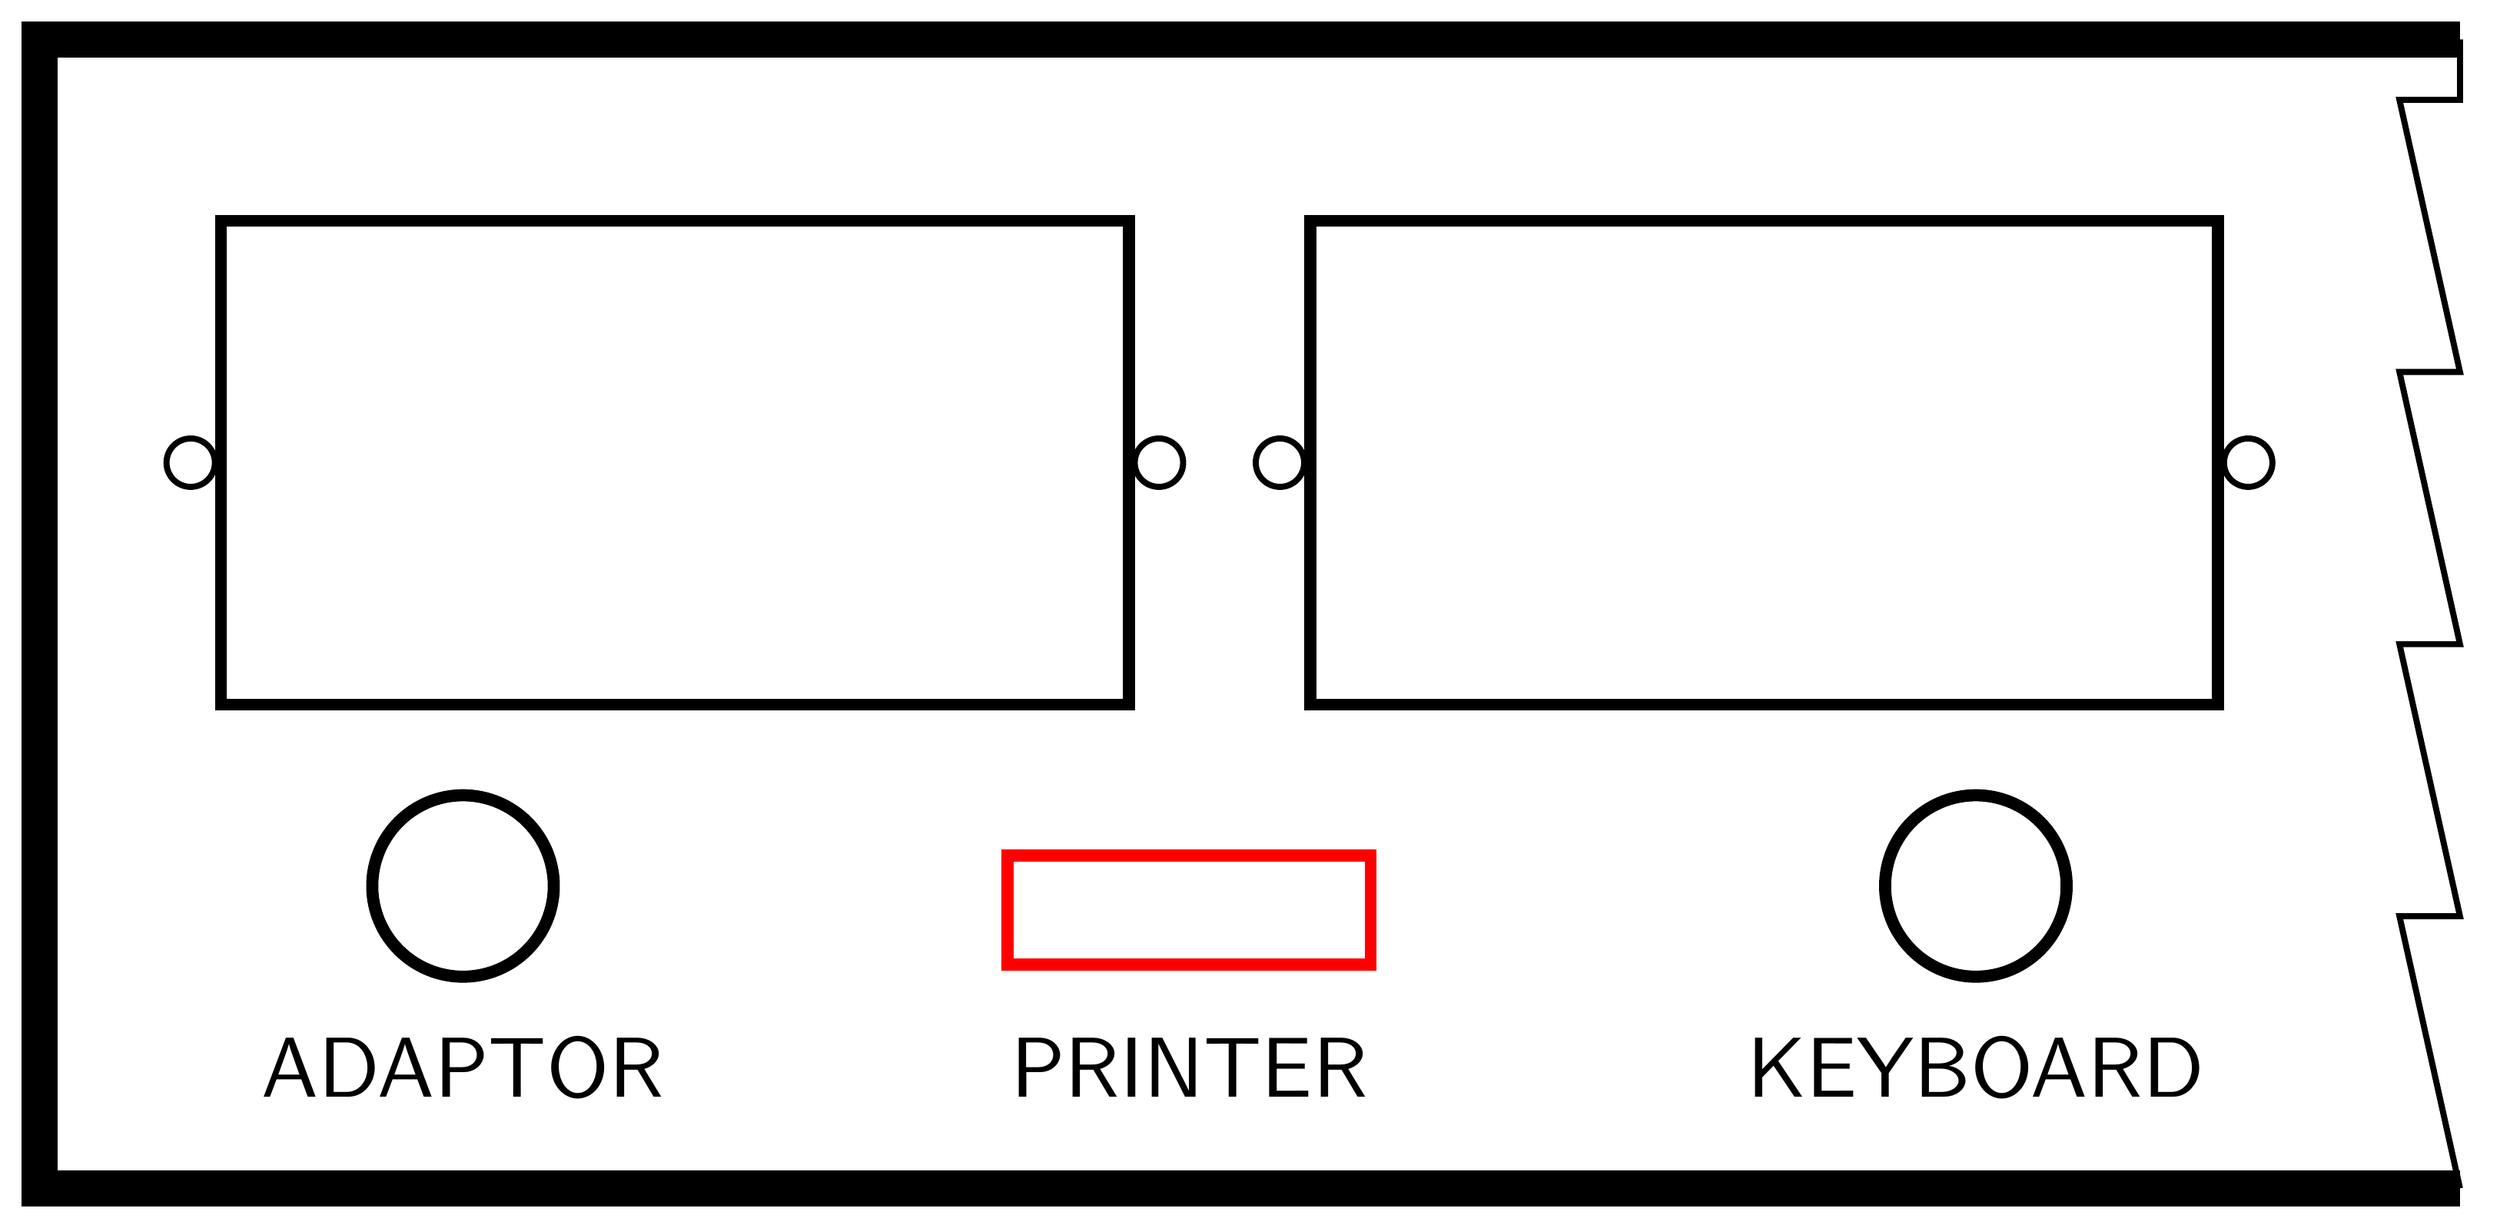
\begin{tikzpicture}[font=\sffamily]
				\draw[line width=6mm] (40,19) -- ++(-40,0) -- ++(0,-19) -- ++(40,0);
				\draw[line width=1mm,decorate,decoration={saw,segment length=45mm,amplitude=10mm}] (40,0) -- ++(0,19);
				\draw[line width=2mm,fill=white] (3,8) rectangle (18,16);
				\draw[line width=2mm,fill=white] (21,8) rectangle (36,16);
				\draw[line width=1mm,fill=white] (2.5,12) circle (4mm);
				\draw[line width=1mm,fill=white] (18.5,12) circle (4mm);
				\draw[line width=1mm,fill=white] (20.5,12) circle (4mm);
				\draw[line width=1mm,fill=white] (36.5,12) circle (4mm);

				\draw[line width=2mm,fill=white] (7,5) circle (15mm);
				\draw[line width=2mm,fill=white] (32,5) circle (15mm);
				\node[black,scale=4] at (7,2) {ADAPTOR};
				\node[black,scale=4] at (32,2) {KEYBOARD};
				\draw[line width=2mm,color=red,fill=white] (16,3.7) rectangle (22,5.5); \node[black,scale=4,] at (19,2) {PRINTER};
			\end{tikzpicture}
		}
		\caption[Keyboard port position.]{NABU Personal Computer \texttt{PRINTER} port.}
		\label{fig:backprt}
	\end{center}
\end{figure}

\begin{figure}[h!]
	\begin{center}
		\scalebox{0.175}{
		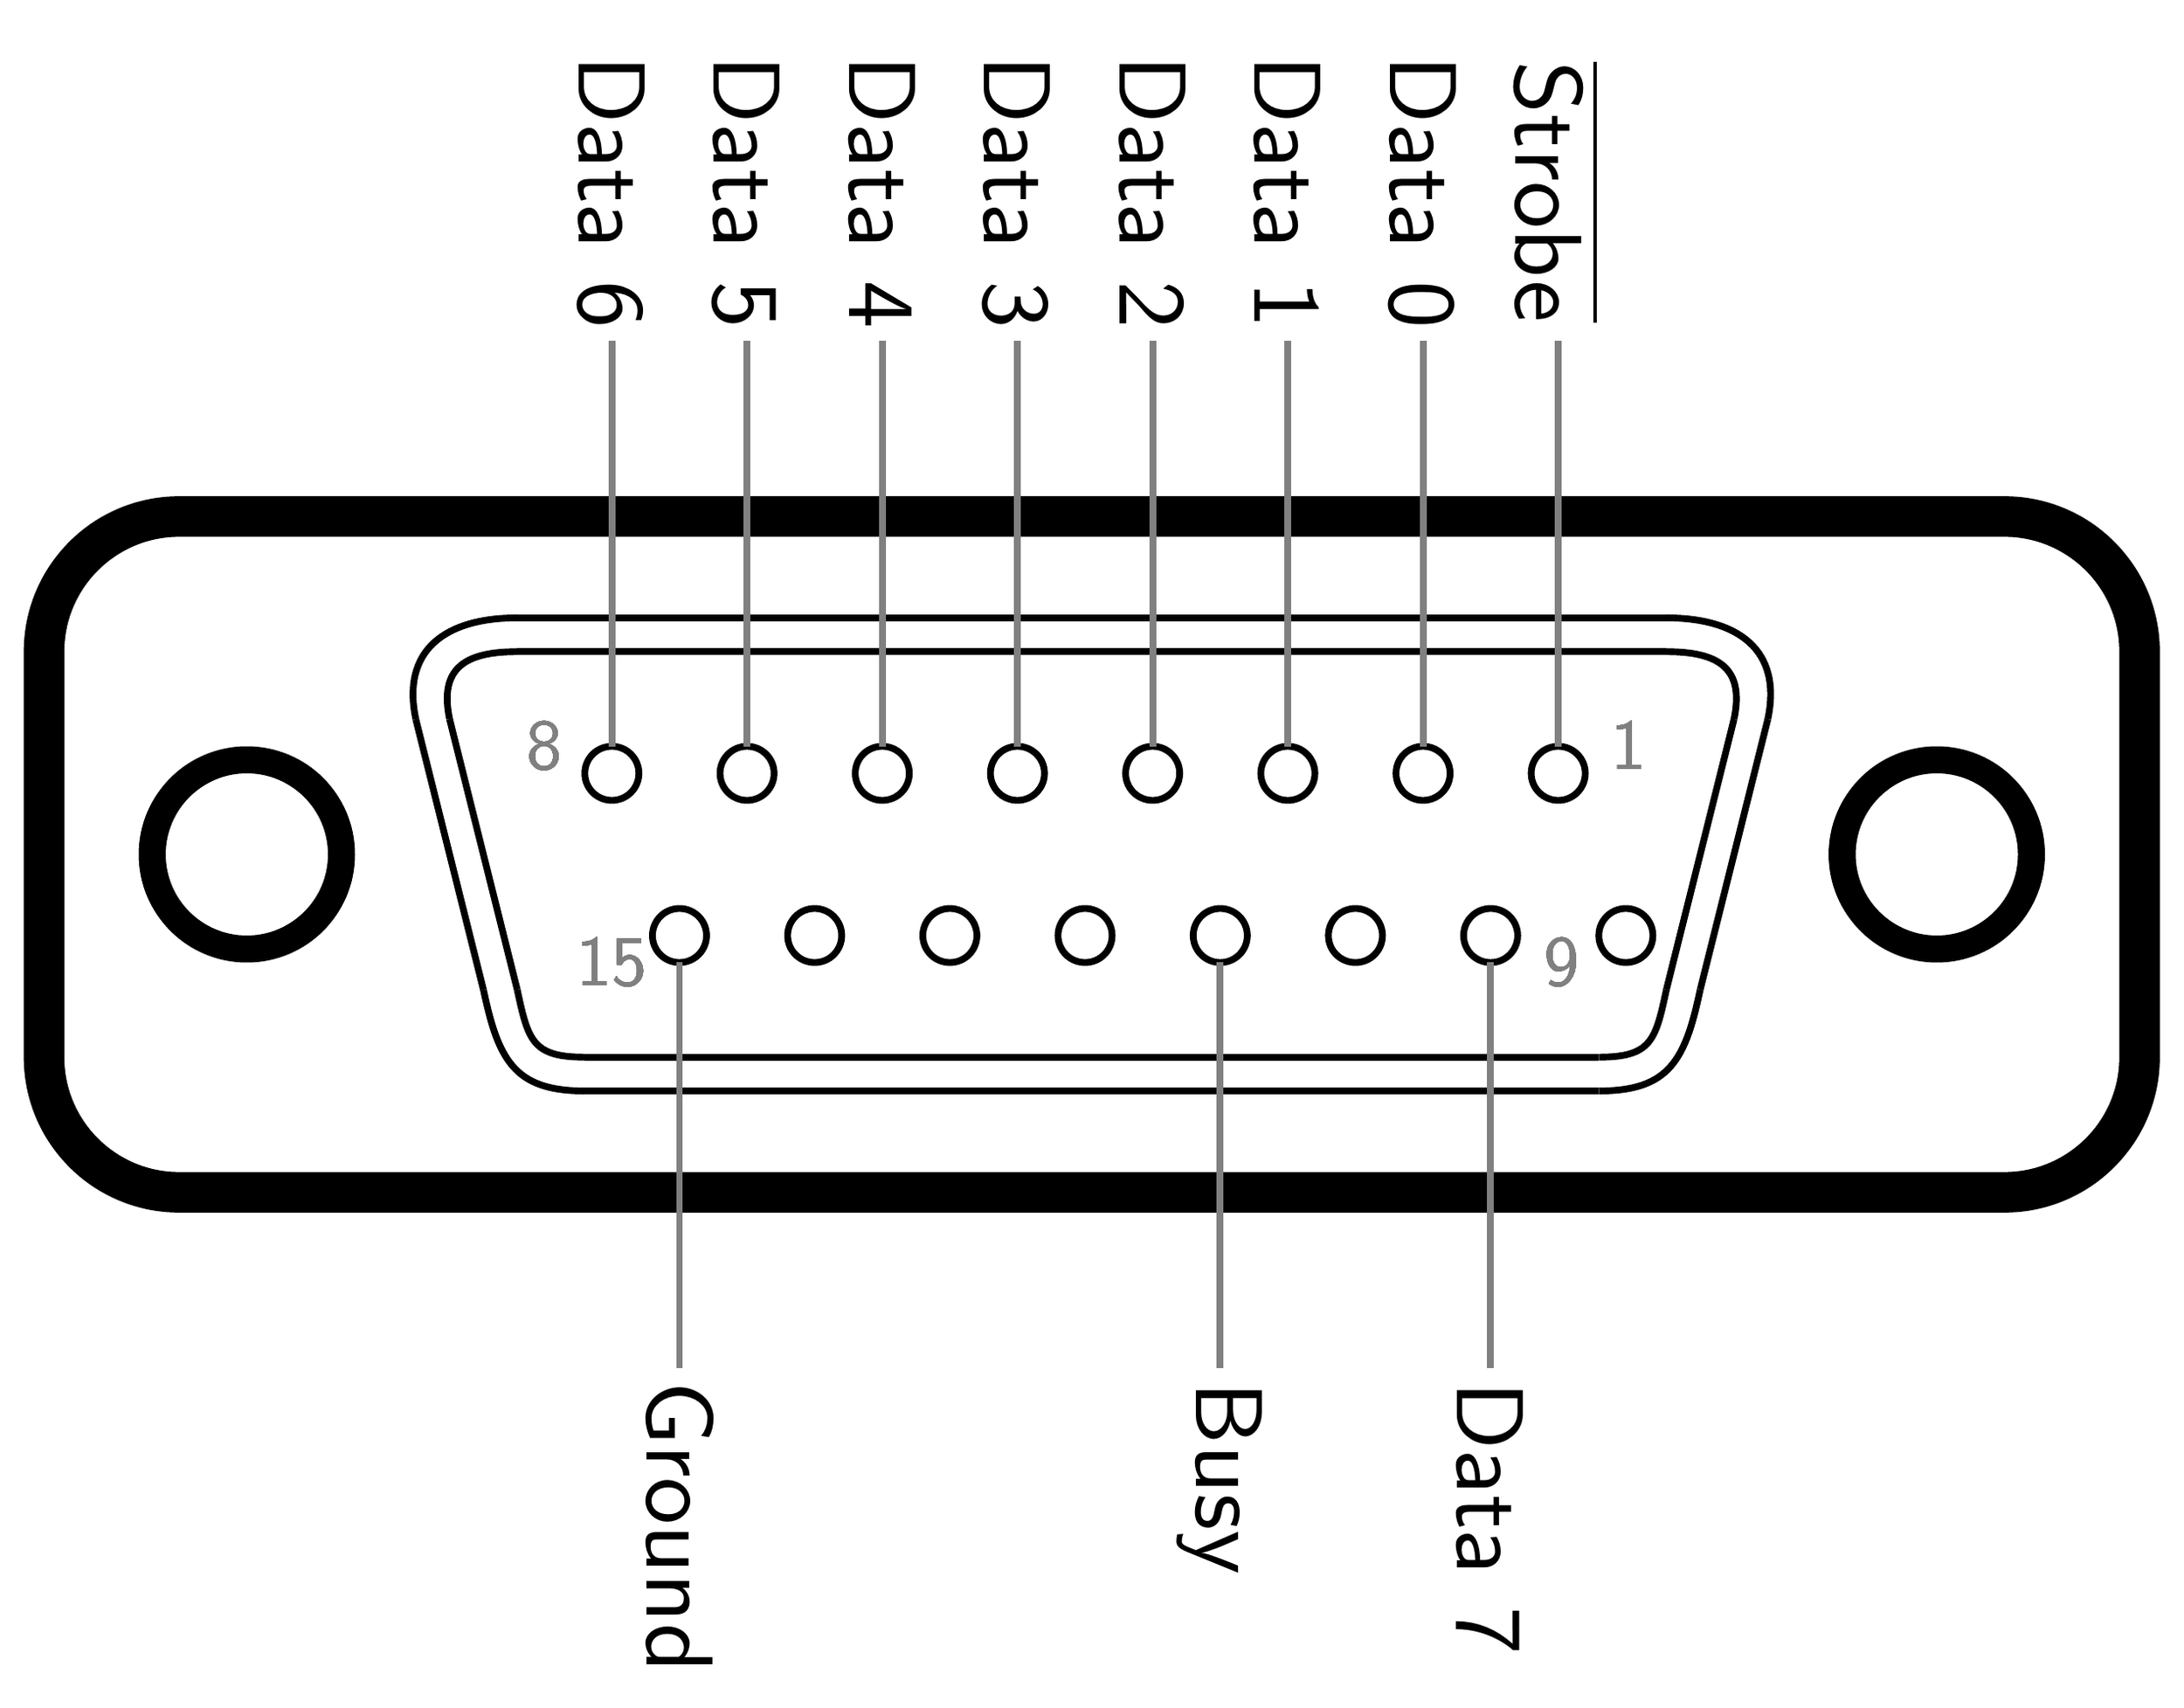
\begin{tikzpicture}[font=\sffamily]
			\draw[rounded corners=2cm,line width=6mm] (0, 0) rectangle (31,10) {};

			\draw[line width=4mm] (3,5) circle (1.4cm);
			\draw[line width=4mm] (28,5) circle (1.4cm);

			\draw[line width=1mm] (7,8) -- (24,8);
			\draw[line width=1mm] (8,2) -- (23,2);
			\draw[line width=1mm] (6,7) -- (7,3);
			\draw[line width=1mm] (25,7) -- (24,3);
			\draw[line width=1mm] (6,7) to[out=102,in=180,distance=22] (7,8);
			\draw[line width=1mm] (7,3) to[out=-78,in=180,distance=22] (8,2);
			\draw[line width=1mm] (23,2) to[out=0,in=-102,distance=22] (24,3);
			\draw[line width=1mm] (25,7) to[out=78,in=0,distance=22] (24,8);

			\draw[line width=1mm] (7,8.5) -- (24,8.5);
			\draw[line width=1mm] (8,1.5) -- (23,1.5);
			\draw[line width=1mm] (5.5,7) -- (6.5,3);
			\draw[line width=1mm] (25.5,7) -- (24.5,3);
			\draw[line width=1mm] (5.5,7) to[out=102,in=180,distance=30] (7,8.5);
			\draw[line width=1mm] (6.5,3) to[out=-78,in=180,distance=30] (8,1.5);
			\draw[line width=1mm] (23,1.5) to[out=0,in=-102,distance=30] (24.5,3);
			\draw[line width=1mm] (25.5,7) to[out=78,in=0,distance=30] (24,8.5);

			\foreach \p\k [count=\q from 0] in {
				{Data~6}/{Ground},{Data~5}/{},{Data~4}/{},{Data~3}/{},{Data~2}/{Busy},{Data~1}/{},{Data~0}/{Data~7},{$\mathsf{\overline{Strobe}}$}/{}} {
				\draw[line width=1mm] (8.4+\q*2,6.2) circle (4mm);
				\ifthenelse{\q<7}{\draw[line width=1mm] (9.4+\q*2,3.8) circle (4mm);	}{}
				\foreach \x in \p {
					\draw[line width=1mm,gray] (8.4+\q*2,6.6) -- ++(0,6);
					\draw (8.4+\q*2,14.8) node[rotate=-90,scale=4]{\p};
				}{}
				\foreach \x in \k {
					\draw[line width=1mm,gray] (9.4+\q*2,3.4) -- ++(0,-6);
					\draw (9.4+\q*2,-4.8) node[rotate=-90,scale=4,text width=1cm]{\k};
				}
				\draw (7.4,6.6) node[scale=3,gray]{8};
				\draw (23.45,6.6) node[scale=3,gray]{1};
				\draw (8.4,3.4) node[scale=3,gray]{15};
				\draw (22.45,3.4) node[scale=3,gray]{9};
			}
		\end{tikzpicture}		}
		\caption[DIN-6 male connector pinouts.]{DB-15 male connector (solder side).}
		\label{fig:din15}
	\end{center}
\end{figure}

\begin{figure}[h!]
  \begin{center}
	\scalebox{0.18}{
		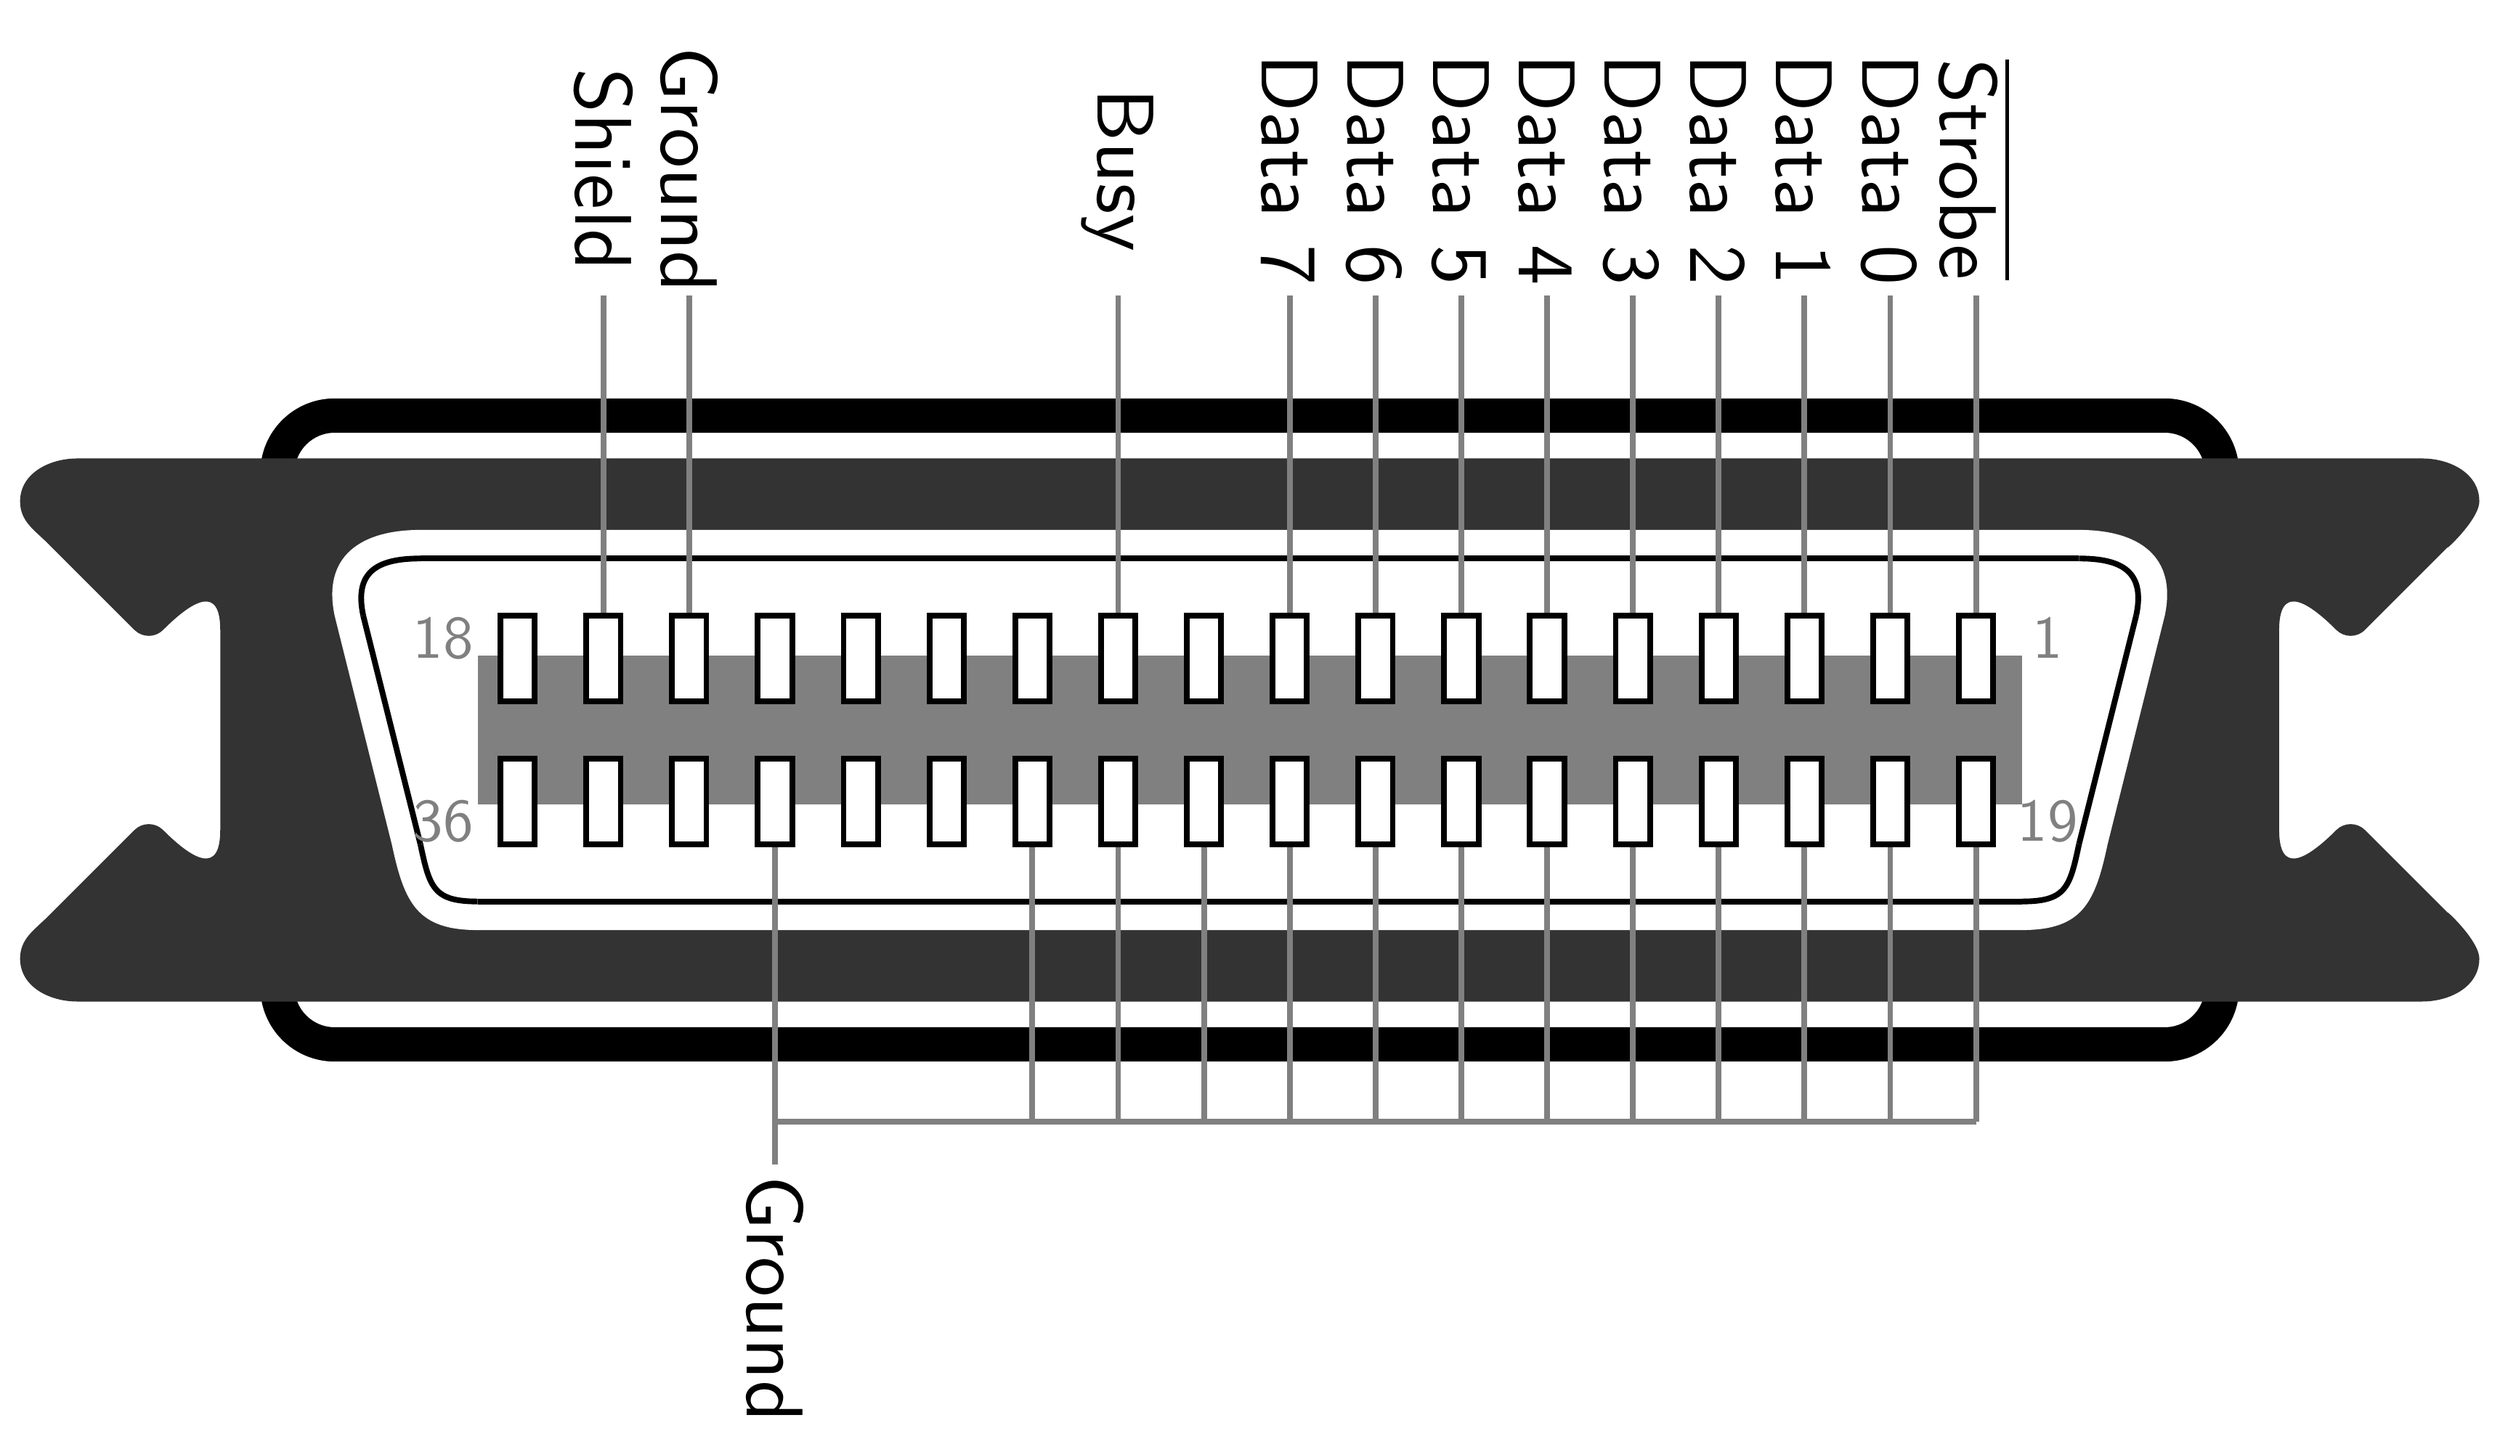
\begin{tikzpicture}[font=\sffamily]
			\draw[rounded corners=1cm,line width=6mm] (.5, -.5) rectangle (34.5,10.5) {};

			\fill[color=black!80,line width=1mm] (-3,9.75) to[out=180,in=90] (-4,9) to[out=-90,in=135] (-3.5,8.25) -- (-2,6.75) to[out=-45,in=225] (-1.5,6.75) to[out=45,in=90,distance=22] (-0.5,6.75) -- (-0.5,3.25) to[out=-90,in=-45,distance=22] (-1.5,3.25) to [out=-225,in=45] (-2,3.25) -- (-3.5,1.75) to[in=90,out=-135] (-4,1) to[in=180,out=270] (-3,0.25) --
			(38,0.25) to [in=270,out=0] (39,1) to[in=135,out=90] (38.5,1.75) -- (37,3.25) to[in=45,out=135] (36.5,3.25) to[in=-90,out=-135,distance=22] (35.5,3.25) -- (35.5,6.75) to[in=135,out=90,distance=22] (36.5,6.75) to [in=-135,out=-45] (37,6.75) -- (38.5,8.25) to[in=-90,out=-135] (39,9) to[in=0,out=90] (38,9.75) -- cycle;

			\fill[line width=1mm,color=white] (3,8.5) -- (32,8.5) to[out=0,in=78,distance=30] (33.5,7) -- (32.5,3) to[in=0,out=-102,distance=30] (31,1.5) -- (4,1.5) to[in=-78,out=180,distance=30] (2.5,3) -- (1.5,7) to[out=102,in=180,distance=30] (3,8.5);

			\draw[line width=1mm] (3,8) -- (32,8);
			\draw[line width=1mm] (4,2) -- (31,2);
			\draw[line width=1mm] (2,7) -- (3,3);
			\draw[line width=1mm] (33,7) -- (32,3);
			\draw[line width=1mm] (2,7) to[out=102,in=180,distance=22] (3,8);
			\draw[line width=1mm] (3,3) to[out=-78,in=180,distance=22] (4,2);
			\draw[line width=1mm] (31,2) to[out=0,in=-102,distance=22] (32,3);
			\draw[line width=1mm] (33,7) to[out=78,in=0,distance=22] (32,8);

			\fill[fill=black!50] (4,3.7) rectangle (31,6.3);
			\foreach \x in {0,1,...,11} {
				\draw[line width=1mm,gray] (13.7+\x*1.5,3.4) -- ++(0,-5.25);
			}
			\draw[line width=1mm,gray] (9.2,-1.85) -- ++(21,0);
			\foreach \p\k [count=\q from 0] in {
				{}/{},{Shield}/{},{Ground}/{},{}/{Ground},{}/{},{}/{},{}/{},{Busy}/{},{}/{},{Data~7}/{},{Data~6}/{},{Data~5}/{},{Data~4}/{},{Data~3}/{},{Data~2}/{},{Data~1}/{},{Data~0}/{},{$\mathsf{\overline{Strobe}}$}/{}}{
				\foreach \x in \p {
					\draw[line width=1mm,gray] (4.7+\q*1.5,6.6) -- ++(0,6);
					\draw (4.7+\q*1.5,14.8) node[rotate=-90,scale=4]{\p};
				}{}
				\foreach \x in \k {
					\draw[line width=1mm,gray] (4.7+\q*1.5,3.4) -- ++(0,-6);
					\draw (4.7+\q*1.5,-4.8) node[rotate=-90,scale=4,text width=1cm]{\k};
				}
				\draw[line width=1mm,fill=white] (4.4+\q*1.5,5.5) rectangle (5+\q*1.5,7);
				\draw[line width=1mm,fill=white] (4.4+\q*1.5,4.5) rectangle (5+\q*1.5,3);
			}
			\draw (3.4,6.6) node[scale=3,gray]{18};
			\draw (31.45,6.6) node[scale=3,gray]{1};
			\draw (3.4,3.4) node[scale=3,gray]{36};
			\draw (31.45,3.4) node[scale=3,gray]{19};
		\end{tikzpicture}
	}
	\caption[Centronics male connector pinouts.]{Centronics male connector (solder side).}
	\label{fig:centronics}
  \end{center}
\end{figure}
